\subsection{Мониторинг программы}

Мониторинг разработанных \texttt{MBean} и виртуальной машины Java выполнялся с использованием утилиты \texttt{JConsole}.

\subsubsection{Подключение к процессу}

На рисунке \ref{fig:jconsole-1} представлен общий вид вкладки \texttt{MBeans} с зарегистрированными \texttt{MBean}.

\begin{figure}[H]
    \centering
    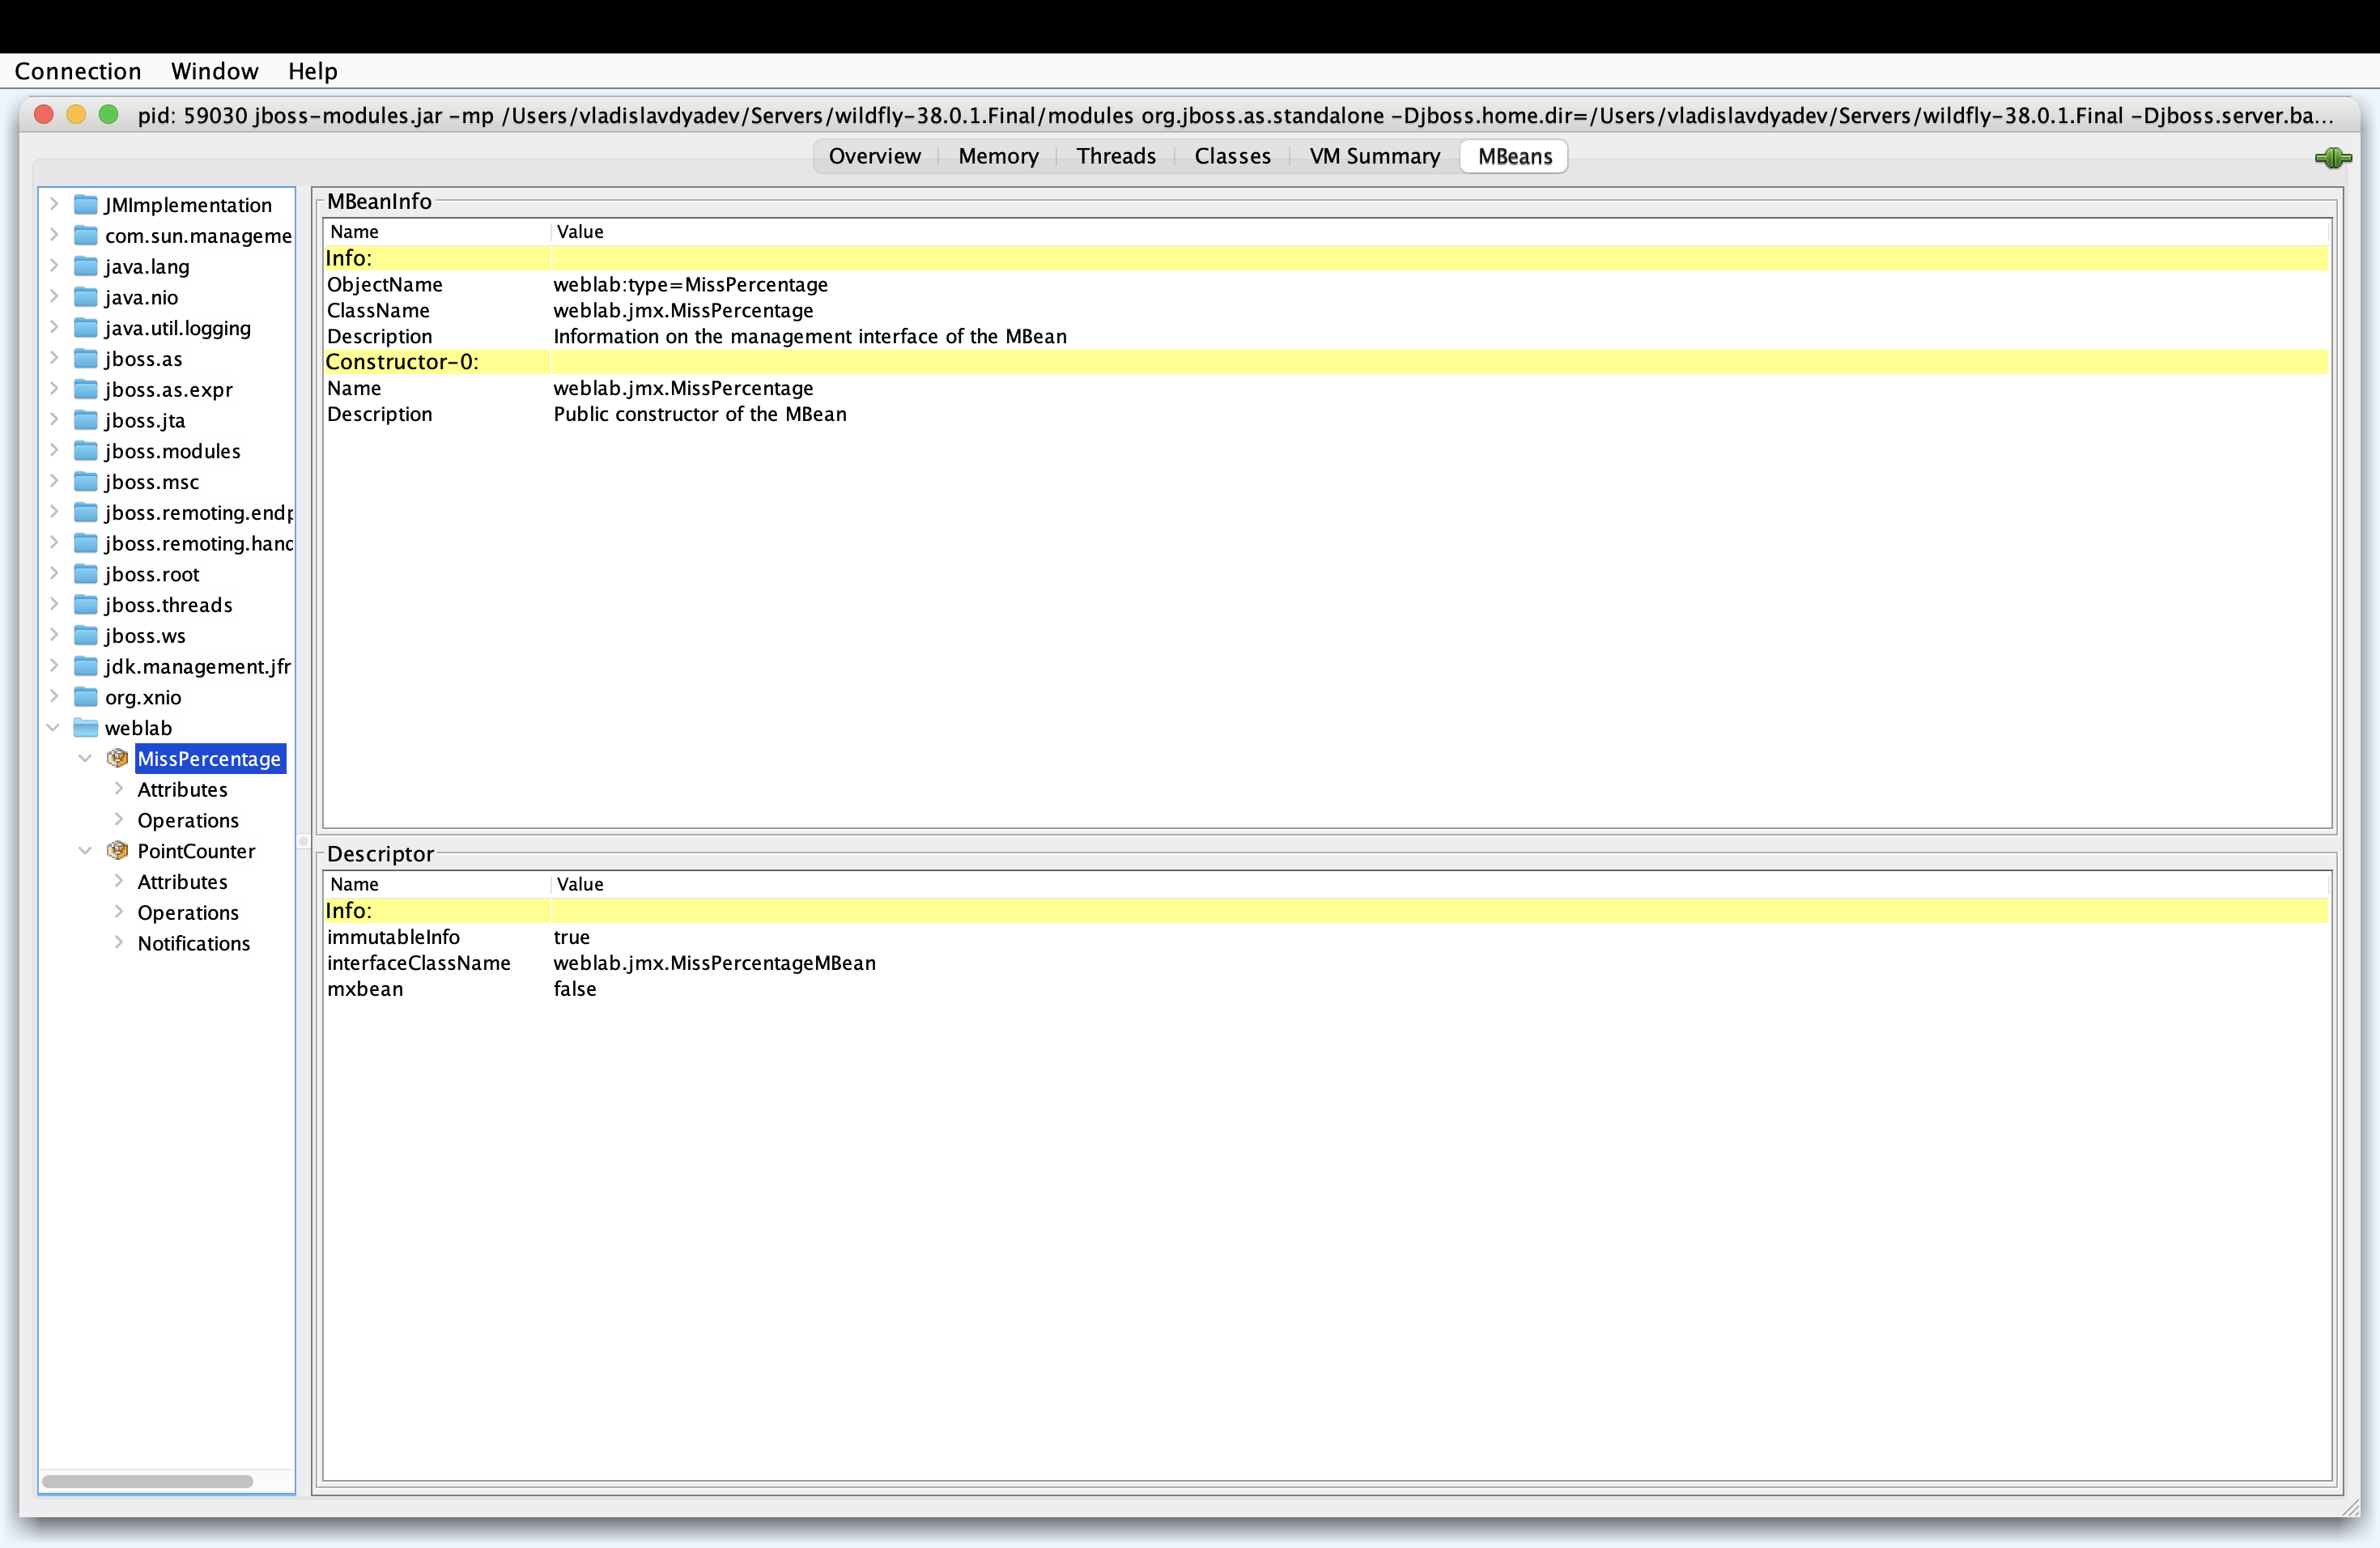
\includegraphics[width=0.7\textwidth]{screenshots/jconsole-1.png}
    \caption{Вкладка \texttt{MBeans} в \texttt{JConsole}.}
    \label{fig:jconsole-1}
\end{figure}

\subsubsection{Мониторинг PointCounter}

MBean \texttt{weblab:type=PointCounter} предоставляет информацию об общем количестве установленных точек и количестве промахов. На рисунке \ref{fig:pointcounter-attributes} показаны показатели и графики изменения значений атрибутов:
\begin{itemize}
    \item \texttt{TotalPoints} — общее количество точек;
    \item \texttt{MissPoints} — количество точек, не попавших в область.
\end{itemize}

\begin{figure}[H]
    \centering
    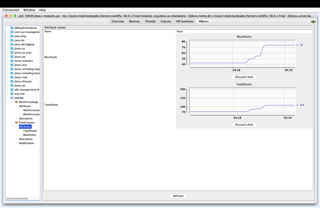
\includegraphics[width=0.7\textwidth]{screenshots/pointcounter-1.png}
    \caption{Атрибуты \texttt{MBean PointCounter}.}
    \label{fig:pointcounter-attributes}
\end{figure}

\subsubsection{Мониторинг MissPercentage}

MBean \texttt{weblab:type=MissPercentage} вычисляет процентное отношение промахов к общему числу кликов. На рисунке \ref{fig:misspercentage-attributes} показаны показатели и график изменения значения атрибута \texttt{MissPercentage}.

\begin{figure}[H]
    \centering
    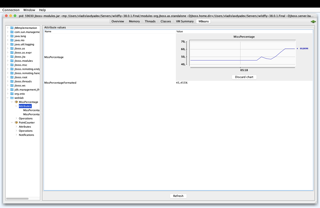
\includegraphics[width=0.7\textwidth]{screenshots/misspercentage.png}
    \caption{Атрибуты \texttt{MBean MissPercentage}.}
    \label{fig:misspercentage-attributes}
\end{figure}

\subsubsection{Уведомления PointCounter}

При достижении общего количества точек, кратного 15, MBean \texttt{PointCounter} отправляет уведомление. На рисунке \ref{fig:notifications} показана вкладка \texttt{Notifications} с зарегистрированными уведомлениями.

\begin{figure}[H]
    \centering
    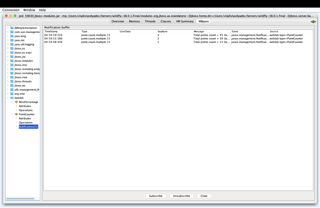
\includegraphics[width=0.7\textwidth]{screenshots/pointcounter-2.png}
    \caption{Уведомления \texttt{MBean PointCounter}.}
    \label{fig:notifications}
\end{figure}

Как видно из рисунка, после 15-го клика было отправлено уведомление с сообщением \texttt{Total points count = 15 (last hit = true)}.

\subsubsection{Информация о виртуальной машине Java}

На вкладке \texttt{VM Summary} была получена следующая информация о виртуальной машине Java (рисунок \ref{fig:vm-summary}):

\begin{itemize}
    \item \textbf{VM Name}: Java HotSpot(TM) 64-Bit Server VM
    \item \textbf{VM Vendor}: Oracle Corporation
    \item \textbf{VM Version}: 23+37-2369
\end{itemize}

\begin{figure}[H]
    \centering
    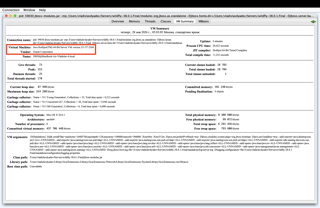
\includegraphics[width=0.7\textwidth]{screenshots/vminfo.png}
    \caption{Информация о виртуальной машине Java.}
    \label{fig:vm-summary}
\end{figure}